\documentclass[letterpaper,10pt,conference]{ieeeconf}

\IEEEoverridecommandlockouts
\overrideIEEEmargins

\usepackage{amsmath,amssymb}
\usepackage{graphicx}
\usepackage{booktabs}
\usepackage{cite}
\usepackage[ruled,vlined]{algorithm2e}
\usepackage{pgfplots}
\usepackage{xcolor}
\usepackage[T1]{fontenc}
\usepackage[utf8]{inputenc}
\pdfsuppresswarningpagegroup=1
\pdfsuppressptexinfo=15
\pgfplotsset{compat=1.18}
\usepgfplotslibrary{groupplots}
\usetikzlibrary{positioning,arrows.meta}
% Auto-generated file. Do not edit manually.
% Generated by scripts/paper/generate_result_macros.py
\providecommand{\CoreAblationFullDelta}{+0.0000}
\providecommand{\CoreAblationFullMean}{0.7510}
\providecommand{\CoreAblationGateHistoryInteractionDelta}{-0.0028}
\providecommand{\CoreAblationGateHistoryInteractionLabel}{worse-than-additive}
\providecommand{\CoreAblationNoGateDelta}{-0.0121}
\providecommand{\CoreAblationNoGateMean}{0.7389}
\providecommand{\CoreAblationNoHistoryDelta}{-0.0306}
\providecommand{\CoreAblationNoHistoryMean}{0.7204}
\providecommand{\CoreAblationNoHistoryNoGateDelta}{-0.0455}
\providecommand{\CoreAblationNoHistoryNoGateMean}{0.7055}
\providecommand{\CoreAblationNoRobustDelta}{-0.0196}
\providecommand{\CoreAblationNoRobustMean}{0.7314}
\providecommand{\CoreAblationVsMainMethodMeanGap}{+0.0016}
\providecommand{\CoreAblationVsMainMethodMeanGapAbs}{0.0016}
\providecommand{\CoreAdversarialDeltaExtTwoMean}{+0.0356}
\providecommand{\CoreAdversarialDeltaExtTwoP}{<0.0001}
\providecommand{\CoreAdversarialExtTwoMean}{0.5122}
\providecommand{\CoreAdversarialExtTwoWorst}{0.4744}
\providecommand{\CoreAdversarialMethodMean}{0.5478}
\providecommand{\CoreAdversarialMethodWorst}{0.5085}
\providecommand{\CoreBinFourHigh}{0.7515}
\providecommand{\CoreBinFourLow}{0.7487}
\providecommand{\CoreBinOneHigh}{0.7431}
\providecommand{\CoreBinOneLow}{0.7403}
\providecommand{\CoreBinThreeHigh}{0.7487}
\providecommand{\CoreBinThreeLow}{0.7459}
\providecommand{\CoreBinTwoHigh}{0.7459}
\providecommand{\CoreBinTwoLow}{0.7431}
\providecommand{\CoreBudgetParityAdaptDeepDeltaEpisodes}{0}
\providecommand{\CoreBudgetParityAdaptDeepDeltaSteps}{0.0}
\providecommand{\CoreBudgetParityAdaptDeepMaxSteps}{0}
\providecommand{\CoreBudgetParityLatencyDeepDeltaEpisodes}{0}
\providecommand{\CoreBudgetParityLatencyDeepDeltaSteps}{0.0}
\providecommand{\CoreBudgetParityLatencyDeepMaxSteps}{0}
\providecommand{\CoreBudgetParityMaxEpisodeDelta}{0}
\providecommand{\CoreBudgetParityMaxExtraMonitorEpisodes}{0}
\providecommand{\CoreBudgetParityMaxMeanStepDelta}{0.000}
\providecommand{\CoreBudgetParityMaxTotalStepDelta}{0.0}
\providecommand{\CoreBudgetParityRows}{4}
\providecommand{\CoreCalibrationMaxAbsError}{0.0010}
\providecommand{\CoreCalibrationTolerance}{0.005}
\providecommand{\CoreCrossEmbodimentDeltaExtTwoCi}{0.0058}
\providecommand{\CoreCrossEmbodimentDeltaExtTwoCvar}{+0.0350}
\providecommand{\CoreCrossEmbodimentDeltaExtTwoD}{1.369}
\providecommand{\CoreCrossEmbodimentDeltaExtTwoMean}{+0.0343}
\providecommand{\CoreCrossEmbodimentDeltaExtTwoP}{<0.0001}
\providecommand{\CoreCrossEmbodimentDeltaExtTwoWorst}{+0.0351}
\providecommand{\CoreCrossEmbodimentDeltaLatencyCi}{0.0056}
\providecommand{\CoreCrossEmbodimentDeltaLatencyCvar}{+0.0291}
\providecommand{\CoreCrossEmbodimentDeltaLatencyD}{1.182}
\providecommand{\CoreCrossEmbodimentDeltaLatencyMean}{+0.0288}
\providecommand{\CoreCrossEmbodimentDeltaLatencyP}{<0.0001}
\providecommand{\CoreCrossEmbodimentDeltaLatencyWorst}{+0.0312}
\providecommand{\CoreCrossEmbodimentExtTwoCvar}{0.4252}
\providecommand{\CoreCrossEmbodimentExtTwoMean}{0.4277}
\providecommand{\CoreCrossEmbodimentExtTwoWorst}{0.4243}
\providecommand{\CoreCrossEmbodimentLatencyAwareCvar}{0.4311}
\providecommand{\CoreCrossEmbodimentLatencyAwareMean}{0.4333}
\providecommand{\CoreCrossEmbodimentLatencyAwareWorst}{0.4283}
\providecommand{\CoreCrossEmbodimentMethodCvar}{0.4601}
\providecommand{\CoreCrossEmbodimentMethodMean}{0.4621}
\providecommand{\CoreCrossEmbodimentMethodWorst}{0.4594}
\providecommand{\CoreCustomBaselineCi}{0.0025}
\providecommand{\CoreCustomBaselineCvar}{0.7095}
\providecommand{\CoreCustomBaselineMean}{0.7119}
\providecommand{\CoreCustomBaselineWorst}{0.7074}
\providecommand{\CoreCustomDeltaExtTwoCi}{0.0027}
\providecommand{\CoreCustomDeltaExtTwoMean}{+0.0054}
\providecommand{\CoreCustomExtOneCi}{0.0009}
\providecommand{\CoreCustomExtOneCvar}{0.7298}
\providecommand{\CoreCustomExtOneMean}{0.7308}
\providecommand{\CoreCustomExtOneWorst}{0.7295}
\providecommand{\CoreCustomExtTwoCi}{0.0022}
\providecommand{\CoreCustomExtTwoCvar}{0.7418}
\providecommand{\CoreCustomExtTwoMean}{0.7440}
\providecommand{\CoreCustomExtTwoWorst}{0.7404}
\providecommand{\CoreCustomMethodCi}{0.0015}
\providecommand{\CoreCustomMethodCvar}{0.7476}
\providecommand{\CoreCustomMethodMean}{0.7494}
\providecommand{\CoreCustomMethodWorst}{0.7474}
\providecommand{\CoreCustomPermComb}{252}
\providecommand{\CoreCustomPermP}{0.0079}
\providecommand{\CoreCustomPermutationPoolN}{10}
\providecommand{\CoreCustomSeedN}{5}
\providecommand{\CoreCvarAlpha}{0.4}
\providecommand{\CoreCvarPercentLabel}{40}
\providecommand{\CoreEnsembleHeads}{5}
\providecommand{\CoreEvalEpisodesPrimary}{400}
\providecommand{\CoreEvalEpisodesRecent}{900}
\providecommand{\CoreEvalGpuHoursPrimary}{0.0}
\providecommand{\CoreExpandedSeedCount}{14}
\providecommand{\CoreFullNFourteenBaselineMean}{0.7127}
\providecommand{\CoreFullNFourteenDeltaExtTwo}{+0.0053}
\providecommand{\CoreFullNFourteenDeltaExtTwoCi}{0.0013}
\providecommand{\CoreFullNFourteenExtOneMean}{0.7300}
\providecommand{\CoreFullNFourteenExtTwoMean}{0.7438}
\providecommand{\CoreFullNFourteenMethodMean}{0.7492}
\providecommand{\CoreGateCycleCount}{0}
\providecommand{\CoreGateNegativeCycleIndex}{2}
\providecommand{\CoreGateNegativeDelta}{-0.0190}
\providecommand{\CoreGatePositiveDeltaMean}{0.0370}
\providecommand{\CoreHeadLayers}{2}
\providecommand{\CoreHeadWidth}{256}
\providecommand{\CoreHistoryHidden}{128}
\providecommand{\CoreHistoryLayers}{2}
\providecommand{\CoreHistoryWindow}{8}
\providecommand{\CoreLatencyParityAvailability}{not-found-public-release}
\providecommand{\CoreLatencyParityStatus}{no-public-repo-subset-verified}
\providecommand{\CoreLatencyProxyPaperCalibStatus}{PASS}
\providecommand{\CoreLatencyProxyPaperGapCvar}{0.0000}
\providecommand{\CoreLatencyProxyPaperGapMax}{0.0000}
\providecommand{\CoreLatencyProxyPaperGapMean}{0.0000}
\providecommand{\CoreLatencyProxyPaperGapWorst}{0.0000}
\providecommand{\CoreLatencySubsetDeltaCvar}{-0.1667}
\providecommand{\CoreLatencySubsetDeltaMean}{-0.0667}
\providecommand{\CoreLatencySubsetDeltaMeanCi}{0.1307}
\providecommand{\CoreLatencySubsetDeltaWorst}{-0.3333}
\providecommand{\CoreLatencySubsetTaskCount}{3}
\providecommand{\CoreLibLaneDRllib}{0.677}
\providecommand{\CoreLibLaneDSbThree}{0.902}
\providecommand{\CoreLibLaneDeltaRllib}{+0.0160}
\providecommand{\CoreLibLaneDeltaSbThree}{+0.0219}
\providecommand{\CoreLibLaneMethodMean}{0.6700}
\providecommand{\CoreLibLaneN}{50}
\providecommand{\CoreLibLanePRllib}{0.000990}
\providecommand{\CoreLibLanePSbThree}{0.000025}
\providecommand{\CoreLibLaneRllibMean}{0.6540}
\providecommand{\CoreLibLaneSbThreeMean}{0.6481}
\providecommand{\CoreLibParityRllibCommit}{a6faf23e6f47}
\providecommand{\CoreLibParitySbThreeCommit}{cc20f5af0cfe}
\providecommand{\CoreLibParityStatus}{PASS}
\providecommand{\CoreMainSeedCount}{5}
\providecommand{\CoreManiDeltaExtTwoCi}{0.0093}
\providecommand{\CoreManiDeltaExtTwoCvar}{+0.0331}
\providecommand{\CoreManiDeltaExtTwoD}{1.233}
\providecommand{\CoreManiDeltaExtTwoMean}{+0.0331}
\providecommand{\CoreManiDeltaExtTwoP}{<0.0001}
\providecommand{\CoreManiDeltaExtTwoWorst}{+0.0323}
\providecommand{\CoreManiDeltaLatencyCi}{0.0096}
\providecommand{\CoreManiDeltaLatencyCvar}{+0.0290}
\providecommand{\CoreManiDeltaLatencyD}{0.989}
\providecommand{\CoreManiDeltaLatencyMean}{+0.0275}
\providecommand{\CoreManiDeltaLatencyP}{<0.0001}
\providecommand{\CoreManiDeltaLatencyWorst}{+0.0335}
\providecommand{\CoreManiExtTwoCvar}{0.3912}
\providecommand{\CoreManiExtTwoMean}{0.3946}
\providecommand{\CoreManiExtTwoWorst}{0.3893}
\providecommand{\CoreManiLatencyAwareCvar}{0.3953}
\providecommand{\CoreManiLatencyAwareMean}{0.4002}
\providecommand{\CoreManiLatencyAwareWorst}{0.3881}
\providecommand{\CoreManiMethodCvar}{0.4243}
\providecommand{\CoreManiMethodMean}{0.4277}
\providecommand{\CoreManiMethodWorst}{0.4216}
\providecommand{\CoreMcSamples}{200,000}
\providecommand{\CoreMetaActiveTaskCount}{9}
\providecommand{\CoreMetaAdaptCvarAlphaHigh}{0.5}
\providecommand{\CoreMetaAdaptCvarAlphaLow}{0.1}
\providecommand{\CoreMetaAdaptCvarAlphaMaxDelta}{+0.2000}
\providecommand{\CoreMetaAdaptCvarAlphaMinDelta}{+0.1733}
\providecommand{\CoreMetaAdaptEqBootstrapSamples}{10000}
\providecommand{\CoreMetaAdaptEqBothLabel}{equivalence-not-established}
\providecommand{\CoreMetaAdaptEqCvarCiNinetyHigh}{+0.2000}
\providecommand{\CoreMetaAdaptEqCvarCiNinetyLow}{+0.0500}
\providecommand{\CoreMetaAdaptEqCvarLabel}{equivalence-not-supported}
\providecommand{\CoreMetaAdaptEqMargin}{0.050}
\providecommand{\CoreMetaAdaptEqMeanCiNinetyHigh}{+0.1214}
\providecommand{\CoreMetaAdaptEqMeanCiNinetyLow}{+0.0357}
\providecommand{\CoreMetaAdaptEqMeanLabel}{equivalence-not-supported}
\providecommand{\CoreMetaAdaptManipCvar}{0.55}
\providecommand{\CoreMetaAdaptManipMean}{0.62}
\providecommand{\CoreMetaAdaptManipWorst}{0.50}
\providecommand{\CoreMetaAdaptSeedexpConfigHashNFourteen}{77b0d402c1b4}
\providecommand{\CoreMetaAdaptSeedexpConfigHashNThirty}{41e6ea5a64d2}
\providecommand{\CoreMetaAdaptTaskLossList}{hammer, reach}
\providecommand{\CoreMetaAdaptTaskLosses}{2}
\providecommand{\CoreMetaAdaptTaskTies}{5}
\providecommand{\CoreMetaAdaptTaskTotal}{10}
\providecommand{\CoreMetaAdaptTaskWinList}{button-press-topdown, push, soccer}
\providecommand{\CoreMetaAdaptTaskWins}{3}
\providecommand{\CoreMetaAllZeroTaskCount}{1}
\providecommand{\CoreMetaAllZeroTaskList}{peg-insert-side}
\providecommand{\CoreMetaBaselineCvar}{0.05}
\providecommand{\CoreMetaBaselineMean}{0.14}
\providecommand{\CoreMetaBaselineSuccPerK}{1.75}
\providecommand{\CoreMetaBaselineWorst}{0.00}
\providecommand{\CoreMetaConstrainedFlowCvar}{0.65}
\providecommand{\CoreMetaConstrainedFlowMean}{0.68}
\providecommand{\CoreMetaConstrainedFlowWorst}{0.60}
\providecommand{\CoreMetaDeepFamilyAlpha}{0.05}
\providecommand{\CoreMetaDeepFamilyHolmAdaptCvarLabel}{Holm-significant}
\providecommand{\CoreMetaDeepFamilyHolmAdaptCvarP}{<0.0001}
\providecommand{\CoreMetaDeepFamilyHolmAdaptCvarSig}{yes}
\providecommand{\CoreMetaDeepFamilyHolmAdaptMeanLabel}{Holm-significant}
\providecommand{\CoreMetaDeepFamilyHolmAdaptMeanP}{0.0007}
\providecommand{\CoreMetaDeepFamilyHolmAdaptMeanSig}{yes}
\providecommand{\CoreMetaDeepFamilyHolmLatencyCvarLabel}{supplementary-only}
\providecommand{\CoreMetaDeepFamilyHolmLatencyCvarP}{0.3523}
\providecommand{\CoreMetaDeepFamilyHolmLatencyCvarSig}{no}
\providecommand{\CoreMetaDeepFamilyHolmLatencyMeanLabel}{supplementary-only}
\providecommand{\CoreMetaDeepFamilyHolmLatencyMeanP}{0.1875}
\providecommand{\CoreMetaDeepFamilyHolmLatencyMeanSig}{no}
\providecommand{\CoreMetaDeepFamilyHolmMinP}{<0.0001}
\providecommand{\CoreMetaDeepFamilyTests}{2}
\providecommand{\CoreMetaDeltaExtTwoActiveMean}{+0.2667}
\providecommand{\CoreMetaDeltaExtTwoCi}{0.1881}
\providecommand{\CoreMetaDeltaExtTwoD}{0.500}
\providecommand{\CoreMetaDeltaExtTwoMean}{+0.2400}
\providecommand{\CoreMetaDeltaExtTwoP}{0.0239}
\providecommand{\CoreMetaExtOneCvar}{0.25}
\providecommand{\CoreMetaExtOneMean}{0.30}
\providecommand{\CoreMetaExtOneSuccPerK}{3.75}
\providecommand{\CoreMetaExtOneWorst}{0.20}
\providecommand{\CoreMetaExtTwoActiveCvar}{0.44}
\providecommand{\CoreMetaExtTwoActiveMean}{0.53}
\providecommand{\CoreMetaExtTwoActiveWorst}{0.33}
\providecommand{\CoreMetaExtTwoCvar}{0.40}
\providecommand{\CoreMetaExtTwoMean}{0.48}
\providecommand{\CoreMetaExtTwoSuccPerK}{6.00}
\providecommand{\CoreMetaExtTwoWorst}{0.30}
\providecommand{\CoreMetaHistoryKeyframeCvar}{0.25}
\providecommand{\CoreMetaHistoryKeyframeMean}{0.46}
\providecommand{\CoreMetaHistoryKeyframeWorst}{0.10}
\providecommand{\CoreMetaHolmSignificant}{2}
\providecommand{\CoreMetaHolmTests}{8}
\providecommand{\CoreMetaLatencyAwareCvar}{0.65}
\providecommand{\CoreMetaLatencyAwareMean}{0.70}
\providecommand{\CoreMetaLatencyAwareWorst}{0.60}
\providecommand{\CoreMetaLatencyCvarAlphaHigh}{0.5}
\providecommand{\CoreMetaLatencyCvarAlphaLow}{0.1}
\providecommand{\CoreMetaLatencyCvarAlphaMaxDelta}{+0.0500}
\providecommand{\CoreMetaLatencyCvarAlphaMinDelta}{+0.0333}
\providecommand{\CoreMetaLatencyTaskLossList}{reach}
\providecommand{\CoreMetaLatencyTaskLosses}{1}
\providecommand{\CoreMetaLatencyTaskTies}{7}
\providecommand{\CoreMetaLatencyTaskTotal}{10}
\providecommand{\CoreMetaLatencyTaskWinList}{button-press-topdown, hammer}
\providecommand{\CoreMetaLatencyTaskWins}{2}
\providecommand{\CoreMetaMethodActiveCvar}{0.72}
\providecommand{\CoreMetaMethodActiveMean}{0.80}
\providecommand{\CoreMetaMethodActiveWorst}{0.67}
\providecommand{\CoreMetaMethodCvar}{0.65}
\providecommand{\CoreMetaMethodMean}{0.72}
\providecommand{\CoreMetaMethodSuccPerK}{9.00}
\providecommand{\CoreMetaMethodWorst}{0.60}
\providecommand{\CoreMetaNFourteenFamilyAlpha}{0.05}
\providecommand{\CoreMetaNFourteenFamilyTests}{2}
\providecommand{\CoreMetaNFourteenHolmAdaptCvarP}{0.0490}
\providecommand{\CoreMetaNFourteenHolmAdaptMeanLabel}{Holm-non-significant}
\providecommand{\CoreMetaNFourteenHolmAdaptMeanP}{0.2068}
\providecommand{\CoreMetaNFourteenHolmAdaptMeanSig}{no}
\providecommand{\CoreMetaNFourteenHolmExtTwoCvarP}{<0.0001}
\providecommand{\CoreMetaNFourteenHolmExtTwoMeanP}{<0.0001}
\providecommand{\CoreMetaNFourteenHolmExtTwoMeanSig}{yes}
\providecommand{\CoreMetaNFourteenHolmLatencyMeanP}{0.1556}
\providecommand{\CoreMetaRobustCpCvar}{0.50}
\providecommand{\CoreMetaRobustCpMean}{0.60}
\providecommand{\CoreMetaRobustCpWorst}{0.40}
\providecommand{\CoreMetaSeedExpAdaptCompCi}{0.0588}
\providecommand{\CoreMetaSeedExpAdaptCompCvar}{0.5167}
\providecommand{\CoreMetaSeedExpAdaptCompMean}{0.6214}
\providecommand{\CoreMetaSeedExpAdaptCompWorst}{0.4000}
\providecommand{\CoreMetaSeedExpAdaptCvarDelta}{+0.1333}
\providecommand{\CoreMetaSeedExpAdaptCvarLabel}{significant}
\providecommand{\CoreMetaSeedExpAdaptCvarSig}{yes}
\providecommand{\CoreMetaSeedExpAdaptD}{0.166}
\providecommand{\CoreMetaSeedExpAdaptDeltaCi}{0.1109}
\providecommand{\CoreMetaSeedExpAdaptDeltaJ}{+0.2052}
\providecommand{\CoreMetaSeedExpAdaptDeltaMean}{+0.0786}
\providecommand{\CoreMetaSeedExpAdaptMeanShrinkDelta}{-0.0581}
\providecommand{\CoreMetaSeedExpAdaptMeanShrinkLabel}{expands}
\providecommand{\CoreMetaSeedExpAdaptMeanShrinkPctAbs}{73.9}
\providecommand{\CoreMetaSeedExpAdaptMethodCi}{0.0356}
\providecommand{\CoreMetaSeedExpAdaptMethodCvar}{0.6500}
\providecommand{\CoreMetaSeedExpAdaptMethodMean}{0.7000}
\providecommand{\CoreMetaSeedExpAdaptMethodWorst}{0.6000}
\providecommand{\CoreMetaSeedExpAdaptN}{14}
\providecommand{\CoreMetaSeedExpAdaptNFourteenPowerCurrent}{0.072}
\providecommand{\CoreMetaSeedExpAdaptNFourteenPowerTarget}{0.8}
\providecommand{\CoreMetaSeedExpAdaptNFourteenPowerTargetN}{571}
\providecommand{\CoreMetaSeedExpAdaptNFourteenSummary}{mixed evidence across metrics: one significant and one non-significant}
\providecommand{\CoreMetaSeedExpAdaptNThirtyCompCvar}{0.4417}
\providecommand{\CoreMetaSeedExpAdaptNThirtyCompMean}{0.5600}
\providecommand{\CoreMetaSeedExpAdaptNThirtyCvarDelta}{+0.1917}
\providecommand{\CoreMetaSeedExpAdaptNThirtyD}{0.285}
\providecommand{\CoreMetaSeedExpAdaptNThirtyDeltaCi}{0.0767}
\providecommand{\CoreMetaSeedExpAdaptNThirtyDeltaJ}{+0.3187}
\providecommand{\CoreMetaSeedExpAdaptNThirtyDeltaMean}{+0.1367}
\providecommand{\CoreMetaSeedExpAdaptNThirtyMethodCvar}{0.6333}
\providecommand{\CoreMetaSeedExpAdaptNThirtyMethodMean}{0.6967}
\providecommand{\CoreMetaSeedExpAdaptNThirtyN}{30}
\providecommand{\CoreMetaSeedExpAdaptNThirtyP}{0.0007}
\providecommand{\CoreMetaSeedExpAdaptNThirtyPCvar}{<0.0001}
\providecommand{\CoreMetaSeedExpAdaptNThirtyPermMcSeCvar}{0.000000}
\providecommand{\CoreMetaSeedExpAdaptNThirtyPermMcSeMean}{0.000059}
\providecommand{\CoreMetaSeedExpAdaptNThirtyPermSamplesCvar}{200000}
\providecommand{\CoreMetaSeedExpAdaptNThirtyPermSamplesMean}{200000}
\providecommand{\CoreMetaSeedExpAdaptNThirtyPowerCurrent}{0.197}
\providecommand{\CoreMetaSeedExpAdaptNThirtyPowerTarget}{0.8}
\providecommand{\CoreMetaSeedExpAdaptNThirtyPowerTargetN}{193}
\providecommand{\CoreMetaSeedExpAdaptNThirtyWorstDelta}{+0.2000}
\providecommand{\CoreMetaSeedExpAdaptP}{0.206820}
\providecommand{\CoreMetaSeedExpAdaptPCvar}{0.049000}
\providecommand{\CoreMetaSeedExpAdaptTwoStageBonfCvarLabel}{Bonferroni-significant}
\providecommand{\CoreMetaSeedExpAdaptTwoStageBonfCvarP}{<0.0001}
\providecommand{\CoreMetaSeedExpAdaptTwoStageBonfMeanLabel}{Bonferroni-significant}
\providecommand{\CoreMetaSeedExpAdaptTwoStageBonfMeanP}{0.0014}
\providecommand{\CoreMetaSeedExpAdaptWorstDelta}{+0.2000}
\providecommand{\CoreMetaSeedExpAdaptWorstDeltaDirection}{positive}
\providecommand{\CoreMetaSeedExpCvarDelta}{+0.2667}
\providecommand{\CoreMetaSeedExpD}{0.553}
\providecommand{\CoreMetaSeedExpDeltaCi}{0.1120}
\providecommand{\CoreMetaSeedExpDeltaJ}{+0.5176}
\providecommand{\CoreMetaSeedExpDeltaMean}{+0.2643}
\providecommand{\CoreMetaSeedExpExtTwoCi}{0.0571}
\providecommand{\CoreMetaSeedExpExtTwoCvar}{0.3500}
\providecommand{\CoreMetaSeedExpExtTwoMean}{0.4429}
\providecommand{\CoreMetaSeedExpExtTwoWorst}{0.3000}
\providecommand{\CoreMetaSeedExpLatencyCompCi}{0.0571}
\providecommand{\CoreMetaSeedExpLatencyCompCvar}{0.5500}
\providecommand{\CoreMetaSeedExpLatencyCompMean}{0.6429}
\providecommand{\CoreMetaSeedExpLatencyCompWorst}{0.4000}
\providecommand{\CoreMetaSeedExpLatencyCvarDelta}{+0.1000}
\providecommand{\CoreMetaSeedExpLatencyD}{0.185}
\providecommand{\CoreMetaSeedExpLatencyDeltaCi}{0.1087}
\providecommand{\CoreMetaSeedExpLatencyDeltaMean}{+0.0857}
\providecommand{\CoreMetaSeedExpLatencyMethodCi}{0.0479}
\providecommand{\CoreMetaSeedExpLatencyMethodCvar}{0.6500}
\providecommand{\CoreMetaSeedExpLatencyMethodMean}{0.7286}
\providecommand{\CoreMetaSeedExpLatencyMethodWorst}{0.6000}
\providecommand{\CoreMetaSeedExpLatencyN}{14}
\providecommand{\CoreMetaSeedExpLatencyNThirtyCompCvar}{0.5667}
\providecommand{\CoreMetaSeedExpLatencyNThirtyCompMean}{0.6600}
\providecommand{\CoreMetaSeedExpLatencyNThirtyCvarDelta}{+0.0500}
\providecommand{\CoreMetaSeedExpLatencyNThirtyD}{0.115}
\providecommand{\CoreMetaSeedExpLatencyNThirtyDeltaCi}{0.0742}
\providecommand{\CoreMetaSeedExpLatencyNThirtyDeltaMean}{+0.0533}
\providecommand{\CoreMetaSeedExpLatencyNThirtyMethodCvar}{0.6167}
\providecommand{\CoreMetaSeedExpLatencyNThirtyMethodMean}{0.7133}
\providecommand{\CoreMetaSeedExpLatencyNThirtyN}{30}
\providecommand{\CoreMetaSeedExpLatencyNThirtyP}{0.1875}
\providecommand{\CoreMetaSeedExpLatencyNThirtyPCvar}{0.3523}
\providecommand{\CoreMetaSeedExpLatencyNThirtyPowerCurrent}{0.073}
\providecommand{\CoreMetaSeedExpLatencyNThirtyPowerTarget}{0.8}
\providecommand{\CoreMetaSeedExpLatencyNThirtyPowerTargetN}{1188}
\providecommand{\CoreMetaSeedExpLatencyNThirtyWorstDelta}{+0.0000}
\providecommand{\CoreMetaSeedExpLatencyP}{0.1556}
\providecommand{\CoreMetaSeedExpLatencyPCvar}{0.1183}
\providecommand{\CoreMetaSeedExpLatencyWorstDelta}{+0.2000}
\providecommand{\CoreMetaSeedExpMethodCi}{0.0522}
\providecommand{\CoreMetaSeedExpMethodCvar}{0.6167}
\providecommand{\CoreMetaSeedExpMethodMean}{0.7071}
\providecommand{\CoreMetaSeedExpMethodWorst}{0.5000}
\providecommand{\CoreMetaSeedExpN}{14}
\providecommand{\CoreMetaSeedExpP}{<0.000100}
\providecommand{\CoreMetaSeedExpPCvar}{<0.000100}
\providecommand{\CoreMetaSeedExpWorstDelta}{+0.2000}
\providecommand{\CoreMetaTaskCount}{10}
\providecommand{\CoreMetaTaskList}{reach, push, button-press, button-press-topdown, faucet-open, hammer, pick-place, soccer, peg-insert-side, push-wall}
\providecommand{\CoreObjectiveLambda}{0.95}
\providecommand{\CoreOtwoODeltaExtTwoMean}{+0.0290}
\providecommand{\CoreOtwoODeltaExtTwoP}{<0.0001}
\providecommand{\CoreOtwoOExtTwoCatastrophic}{0.37}
\providecommand{\CoreOtwoOExtTwoInterventions}{3.08}
\providecommand{\CoreOtwoOExtTwoMean}{0.6599}
\providecommand{\CoreOtwoOMethodCatastrophic}{0.27}
\providecommand{\CoreOtwoOMethodInterventions}{3.57}
\providecommand{\CoreOtwoOMethodMean}{0.6889}
\providecommand{\CorePermUpperBound}{0.000005}
\providecommand{\CorePermUpperBoundSci}{5\times10^{-6}}
\providecommand{\CorePropTwoProxyHoldRateAdapt}{0.167}
\providecommand{\CorePropTwoProxyHoldRateLatency}{0.333}
\providecommand{\CorePropTwoProxyHoldRateOverall}{0.250}
\providecommand{\CorePropTwoProxyPairsAdapt}{84}
\providecommand{\CorePropTwoProxyPairsLatency}{84}
\providecommand{\CorePropTwoProxyPairsOverall}{168}
\providecommand{\CorePropTwoProxyViolationRateAdapt}{0.833}
\providecommand{\CorePropTwoProxyViolationRateLatency}{0.667}
\providecommand{\CorePropTwoProxyViolationRateOverall}{0.750}
\providecommand{\CoreRecentComparatorCount}{5}
\providecommand{\CoreRecentHolmSignificant}{3}
\providecommand{\CoreRecentHolmTests}{8}
\providecommand{\CoreRepoVersion}{0.3.6}
\providecommand{\CoreRobustSeedCount}{3}
\providecommand{\CoreRoneDropLimitPct}{10}
\providecommand{\CoreRoneMedMethodDropPct}{4.57\%}
\providecommand{\CoreRthreeSevereBaselineMean}{0.6453}
\providecommand{\CoreRthreeSevereMethodMean}{0.6950}
\providecommand{\CoreRtwoDropLimitPct}{12}
\providecommand{\CoreRtwoMedMethodDropPct}{4.75\%}
\providecommand{\CoreSampleBaselineStepsPerSuccess}{571.4}
\providecommand{\CoreSampleBaselineSuccPerK}{1.75}
\providecommand{\CoreSampleBaselineSuccessTasks}{4}
\providecommand{\CoreSampleBaselineTaskCount}{10}
\providecommand{\CoreSampleExtOneStepsPerSuccess}{266.7}
\providecommand{\CoreSampleExtOneSuccPerK}{3.75}
\providecommand{\CoreSampleExtOneSuccessTasks}{6}
\providecommand{\CoreSampleExtOneTaskCount}{10}
\providecommand{\CoreSampleExtTwoStepsPerSuccess}{166.7}
\providecommand{\CoreSampleExtTwoSuccPerK}{6.00}
\providecommand{\CoreSampleExtTwoSuccessTasks}{8}
\providecommand{\CoreSampleExtTwoTaskCount}{10}
\providecommand{\CoreSampleMethodStepsPerSuccess}{111.1}
\providecommand{\CoreSampleMethodSuccPerK}{9.00}
\providecommand{\CoreSampleMethodSuccessTasks}{9}
\providecommand{\CoreSampleMethodTaskCount}{10}
\providecommand{\CoreSeedExpCvarDelta}{+0.0068}
\providecommand{\CoreSeedExpDeltaMean}{+0.0064}
\providecommand{\CoreSeedExpExtTwoCi}{0.0014}
\providecommand{\CoreSeedExpExtTwoCvar}{0.7403}
\providecommand{\CoreSeedExpExtTwoMean}{0.7429}
\providecommand{\CoreSeedExpExtTwoWorst}{0.7392}
\providecommand{\CoreSeedExpMethodCi}{0.0011}
\providecommand{\CoreSeedExpMethodCvar}{0.7471}
\providecommand{\CoreSeedExpMethodMean}{0.7493}
\providecommand{\CoreSeedExpMethodWorst}{0.7462}
\providecommand{\CoreSeedExpN}{14}
\providecommand{\CoreSeedExpWorstDelta}{+0.0070}
\providecommand{\CoreSimIsaacBaselineMean}{0.6258}
\providecommand{\CoreSimIsaacDelta}{+0.0509}
\providecommand{\CoreSimIsaacDeltaExtTwo}{+0.0108}
\providecommand{\CoreSimIsaacDeltaLatencyAware}{+0.0101}
\providecommand{\CoreSimIsaacExtTwoMean}{0.6659}
\providecommand{\CoreSimIsaacLatencyAwareMean}{0.6666}
\providecommand{\CoreSimIsaacLatencyAwareRetentionPct}{89.9}
\providecommand{\CoreSimIsaacMethodMean}{0.6767}
\providecommand{\CoreSimIsaacMethodRetentionPct}{90.3}
\providecommand{\CoreSimIsaacRetentionGapVsLatencyPct}{+0.4}
\providecommand{\CoreSimMujocoBaselineMean}{0.7122}
\providecommand{\CoreSimMujocoDelta}{+0.0365}
\providecommand{\CoreSimMujocoDeltaExtTwo}{+0.0055}
\providecommand{\CoreSimMujocoDeltaLatencyAware}{+0.0070}
\providecommand{\CoreSimMujocoExtTwoMean}{0.7432}
\providecommand{\CoreSimMujocoLatencyAwareMean}{0.7417}
\providecommand{\CoreSimMujocoLatencyAwareRetentionPct}{100.0}
\providecommand{\CoreSimMujocoMethodMean}{0.7487}
\providecommand{\CoreSimMujocoMethodRetentionPct}{99.9}
\providecommand{\CoreSimSeedCount}{14}
\providecommand{\CoreSoneHardBaselineMean}{0.5884}
\providecommand{\CoreSoneHardMethodMean}{0.6436}
\providecommand{\CoreSthreeDropLimitPct}{18}
\providecommand{\CoreSthreeSevereBaselineMean}{0.6444}
\providecommand{\CoreSthreeSevereMethodDropPct}{7.13\%}
\providecommand{\CoreSthreeSevereMethodMean}{0.6959}
\providecommand{\CoreStwoDropLimitPct}{12}
\providecommand{\CoreStwoMedMethodDropPct}{4.93\%}
\providecommand{\CoreTailNFiveDenominator}{5}
\providecommand{\CoreTailNFiveExtTwo}{1}
\providecommand{\CoreTailNFiveMethod}{0}
\providecommand{\CoreTailNFourteenCvarDelta}{+0.0050}
\providecommand{\CoreTailNFourteenDenominator}{14}
\providecommand{\CoreTailNFourteenExtTwo}{1}
\providecommand{\CoreTailNFourteenMethod}{0}
\providecommand{\CoreTailThreshold}{0.7420}
\providecommand{\CoreTauGreen}{0.02}
\providecommand{\CoreTauRowFourGreen}{0.04}
\providecommand{\CoreTauRowFourGreenCount}{1}
\providecommand{\CoreTauRowFourRedCount}{1}
\providecommand{\CoreTauRowFourYellow}{0.020}
\providecommand{\CoreTauRowFourYellowCount}{8}
\providecommand{\CoreTauRowOneGreen}{0.02}
\providecommand{\CoreTauRowOneGreenCount}{9}
\providecommand{\CoreTauRowOneRedCount}{1}
\providecommand{\CoreTauRowOneYellow}{0.005}
\providecommand{\CoreTauRowOneYellowCount}{0}
\providecommand{\CoreTauRowThreeGreen}{0.04}
\providecommand{\CoreTauRowThreeGreenCount}{1}
\providecommand{\CoreTauRowThreeRedCount}{1}
\providecommand{\CoreTauRowThreeYellow}{0.005}
\providecommand{\CoreTauRowThreeYellowCount}{8}
\providecommand{\CoreTauRowTwoGreen}{0.02}
\providecommand{\CoreTauRowTwoGreenCount}{9}
\providecommand{\CoreTauRowTwoRedCount}{1}
\providecommand{\CoreTauRowTwoYellow}{0.020}
\providecommand{\CoreTauRowTwoYellowCount}{0}
\providecommand{\CoreTauSweepGreenSet}{0.01,0.02,0.04}
\providecommand{\CoreTauSweepYellowSet}{0.003,0.005,0.01,0.02}
\providecommand{\CoreTauYellow}{0.005}
\providecommand{\CoreTheoryNeffAdaptEstimate}{300.0}
\providecommand{\CoreTheoryNeffAdaptIcc}{0.000}
\providecommand{\CoreTheoryNeffAdaptPairs}{300}
\providecommand{\CoreTheoryNeffLatencyEstimate}{300.0}
\providecommand{\CoreTheoryNeffLatencyIcc}{0.000}
\providecommand{\CoreTheoryNeffLatencyPairs}{300}
\providecommand{\CoreTheoryNeffMaxIcc}{0.000}
\providecommand{\CoreTheoryNeffMinEstimate}{300.0}
\providecommand{\CoreTheoryNeffMinFloor}{300}
\providecommand{\CoreTheoryNeffMinPairs}{300}
\providecommand{\CoreTheoryNeffMinRatio}{1.000}
\providecommand{\CoreTheoryNeffRows}{2}
\providecommand{\CoreUncertaintyCoveragePct}{94.5}
\providecommand{\CoreUncertaintyCu}{1.0191}
\providecommand{\CoreUncertaintyCzero}{0.0041}
\providecommand{\CoreUncertaintyHoldoutMae}{0.0049}
\providecommand{\CoreUncertaintyHoldoutRmse}{0.0058}
\providecommand{\CoreUncertaintyHoldoutRows}{510}
\providecommand{\CoreUncertaintyMaxViolation}{0.0063}
\providecommand{\CoreUncertaintyMisspecBaseAcceptRate}{0.945}
\providecommand{\CoreUncertaintyMisspecGridN}{25}
\providecommand{\CoreUncertaintyMisspecMaxFalseAccept}{0.055}
\providecommand{\CoreUncertaintyMisspecMaxFalseReject}{0.945}
\providecommand{\CoreUncertaintyMisspecWorstAgreement}{0.055}
\providecommand{\CoreUncertaintyPearson}{0.9973}
\providecommand{\CoreUncertaintySlope}{0.9904}
\providecommand{\CoreUncertaintyTrainRows}{474}
\providecommand{\CoreUncertaintyViolationPairs}{84}
\providecommand{\CoreUncertaintyViolationRate}{0.833}
\providecommand{\CoreUncertaintyViolationRatePct}{83.3}
\providecommand{\CoreVerificationExtTwoPassRatio}{1.000}
\providecommand{\CoreVerificationFailureFloor}{0}
\providecommand{\CoreVerificationFailureRecovery}{0}
\providecommand{\CoreVerificationFailureStability}{0}
\providecommand{\CoreVerificationMethodGrade}{A}
\providecommand{\CoreVerificationMethodPassRatio}{1.000}

\newtheorem{theorem}{Theorem}
\newtheorem{proposition}{Proposition}
\newtheorem{designlemma}{Design Lemma}
\newtheorem{heuristic}{Diagnostic Heuristic}
\newtheorem{corollary}{Corollary}
\newcommand{\CoreRefOneLabel}{TRPO-U}
\newcommand{\CoreRefTwoLabel}{PPO-CVaR}
\newcommand{\CoreProfileExtOne}{ext1}
\newcommand{\CoreProfileExtTwo}{ext2}
\newcommand{\CoreCompLatencyAware}{LatencyAware}
\newcommand{\CoreCompAdaptManip}{AdaptManip}
\newcommand{\CoreCompRobustCp}{Robust-CP}
\newcommand{\CoreCompHistoryKeyframe}{History-Keyframe}
\newcommand{\CoreCompConstrainedFlow}{Constrained-Flow}
\newcommand{\CoreGatePromote}{promote}
\newcommand{\CoreGateMonitor}{monitor}
\newcommand{\CoreGateRollback}{rollback}
\newcommand{\CoreEnvMujoco}{Mujoco}
\newcommand{\CoreEnvIsaac}{Isaac}
\newcommand{\AnonRepoPlaceholder}{\texttt{[ANON\_REPO\_URL\_TO\_BE\_REVEALED]}}
\newcommand{\CorePaperTitleText}{CORE: Uncertainty-Gated Policy Optimization for Reliable Performance Under Distribution Shift}

\definecolor{coreInk}{HTML}{0F172A}
\definecolor{coreBaseline}{HTML}{7A8896}
\definecolor{coreRefA}{HTML}{59A14F}
\definecolor{coreRefB}{HTML}{F28E2B}
\definecolor{coreMethod}{HTML}{D62728}
\definecolor{coreGrid}{HTML}{B8C7DA}

\pgfplotsset{
    coreplot/.style={
        axis line style={color=coreInk},
        tick style={color=coreInk},
        tick label style={font=\scriptsize,color=coreInk},
        label style={font=\scriptsize,color=coreInk},
        grid style={color=coreGrid},
    }
}

\title{\LARGE \bf \CorePaperTitleText}

\author{
    Shawn Azdam$^{1}$%
    \thanks{$^{1}$Aureuma AI, NYC.}%
    \thanks{Correspondence to: \texttt{shawn@aureuma.ai}}
}

\begin{document}
\maketitle
\thispagestyle{empty}
\pagestyle{empty}

\begin{abstract}
We present Conservative Online Reliability Enforcement (CORE), an uncertainty-gated policy optimization framework for robust policy updates under distribution shift. The method combines risk-aware trust-region learning with online promote/monitor/rollback control driven by uncertainty-calibrated signals. Across matched-seed benchmark and scenario-model evaluations, our approach improves reliability-floor behavior while preserving fixed-budget update control. We provide algorithm design, theory-guided gate rationale, and diagnostics that clarify where gated updates help and where limitations remain.
\end{abstract}


\section{Introduction}

Reliable policy optimization under distribution shift is still a core failure mode in robotics learning systems. Modest changes in latency, sensing quality, or scene geometry can destabilize updates that appear safe under nominal evaluation. Recent work improves planning-time safety and shift robustness \cite{a2602_12047v1,a2602_12616v1,a2602_12032v1,a2602_09021v1}, but update-time rollback control is less explicitly specified.

Our approach addresses this gap with an uncertainty-gated policy optimization loop. It combines a trust-region surrogate update, an ensemble-disagreement penalty, and an online promote/monitor/rollback gate driven by a conservative lower-bound proxy. The novelty is update-time control: unstable candidates are rejected before downstream validation.

On the MetaWorld shifted suite \cite{yu2020metaworld}, Section IV anchors primary confirmatory claims to \CoreRefTwoLabel\ and reports \CoreCompAdaptManip\ as an exploratory paper-profile sensitivity lane with explicit fairness caveats. Mean remains secondary/sensitivity-only, and $N=30$ is sensitivity-only with smaller mean deltas. The unofficial \CoreCompLatencyAware\ proxy lane remains supplementary-only and excluded from primary claim tables.

Contributions are:
\begin{enumerate}
    \item An uncertainty-gated update rule that combines risk-aware trust-region optimization with per-iteration promote/monitor/rollback control.
    \item A floor-focused theory package with one calibration-conditional deployed-gate design lemma plus diagnostic heuristic envelopes (optional one-sided and false-promote sketches) and matched-seed empirical-floor diagnostics.
    \item A reliability-first evidence package with matched-seed diagnostics, targeted seed expansion, ablations, robustness checks, and explicit scope boundaries.
\end{enumerate}

This study focuses on update-time robustness under controlled perturbations. Evidence is simulation-only, and we do not claim deployment-ready safety, hardware validation, or real-robot transfer guarantees.

\section{Related Work}

Recent work improves contact grounding, long-horizon world-model planning, and distribution-shift robustness \cite{a2602_13833v1,a2602_14174v1,a2602_12532v1,a2602_12063v2,a2602_13977v1,a2602_10983v2,a2602_12047v1,a2602_12616v1,a2602_09021v1}. These advances are complementary to our setting, but most intervene at planning/calibration time or through implicit policy-selection loops rather than explicit update-time commit control.

Sim-to-real and policy-scaling foundations define the current baseline bar \cite{tobin2017domain,kalashnikov2018qtopt,andrychowicz2018dexterous,mandlekar2021robomimic,brohan2022rt1,brohan2023rt2,openx2024rtx,chi2023diffusionpolicy}. The unresolved gap for this paper is a conservative, online reject/commit rule for policy updates under fixed evaluation budgets.

Our method is positioned as a policy-optimization method: uncertainty-penalized trust-region updates with an explicit online promote/monitor/rollback gate. Compared with nearby alternatives, the main distinction is update-time rollback control rather than planning-time calibration or model-scale expansion \cite{a2602_12047v1,a2602_12616v1,a2602_12063v2,a2602_13977v1,a2602_10983v2,a2602_12532v1,a2602_14174v1,a2602_15010v1}.
In this comparison set, prior lines emphasize planning-time safety proxies or implicit update selection, while our approach uses explicit promote/monitor/rollback control inside the policy-update loop under matched-seed validation.

\section{Theory and Design Rationale}
This section states one deployed-gate design lemma plus diagnostic heuristic envelopes (optional one-sided false-promote sketch and matched-seed floor remark) that motivate when the gate should promote or reject candidate updates. These are assumption-scoped design-rationale bounds, not claims of new concentration theory.

We consider partially observed control under distribution shift. Let latent state be $s_t \in \mathcal{S}$, observation $o_t \in \mathcal{O}$, action $a_t \in \mathcal{A}$, and history $h_t=(o_{0:t},a_{0:t-1})$. A policy $\pi_\theta(a_t\mid h_t)$ induces trajectory $\tau$ under shift condition $\xi \sim p(\xi)$.

We optimize a risk-aware objective
\begin{equation}
\begin{aligned}
J(\theta) =\;& \mathbb{E}_{\xi \sim p(\xi),\,\tau \sim p(\cdot \mid \pi_\theta,\xi)}\!\left[\sum_{t=0}^{T} \gamma^t r_t\right] \\
&- \lambda\,\mathrm{CVaR}_{\alpha,\;(\tau,\xi)\sim p_\theta}\!\left(-R(\tau,\xi)\right),
\end{aligned}
\label{eq:risk-objective}
\end{equation}
where $p_\theta(\tau,\xi):=p(\xi)\,p(\tau\mid\pi_\theta,\xi)$, $R(\tau,\xi)=\sum_{t=0}^{T}\gamma^t r_t$, $\lambda\ge 0$ controls robustness, and $\alpha$ sets the tail-risk level. We use $\alpha=\CoreCvarAlpha$ (reported as CVaR$_{\CoreCvarPercentLabel}$).
For gate bounds, we separately analyze the return component
\[
G(\theta):=\mathbb{E}_{\xi\sim p(\xi),\,\tau\sim p(\cdot\mid\pi_\theta,\xi)}\!\left[\sum_{t=0}^{T}\gamma^t r_t\right],
\]
while CVaR remains part of the optimization objective in Eq.~\ref{eq:risk-objective}.

At iteration $k$, our method maintains policy parameters $\theta_k$, world-model parameters $\phi_k$, and an uncertainty functional induced by ensemble value disagreement. Let $\{Q_{\phi_k}^{(m)}\}_{m=1}^{M}$ be $M$ bootstrap value heads. For candidate policy $\pi_\theta$ under ensemble snapshot $\phi_k$, define
\begin{equation}
\begin{aligned}
\widehat{U}^{\mathrm{wm}}_k(\theta)
={}&\frac{1}{|\widetilde{\mathcal{S}}_k|}\sum_{i\in\widetilde{\mathcal{S}}_k}
\frac{1}{|\tau_k^{\theta,(i)}|}\sum_t
\mathrm{Var}_{m}\!\left(Q_{\phi_k}^{(m)}(h_t,a_t)\right),
\end{aligned}
\label{eq:uncertainty-score}
\end{equation}
Here $\widetilde{\mathcal{S}}_k:=\widetilde{\mathcal{S}}_k(\theta)$ is a short candidate-policy rollout set produced by world-model snapshot $\phi_k$ from seed-matched incumbent replay starts; gating does not require hardware execution of the candidate policy. $\mathrm{Var}_m(\cdot)$ is the sample variance across the $M$ ensemble heads at fixed $(h_t,a_t)$.
Inspired by recent robust planning and world-model work \cite{a2602_12047v1,a2602_12616v1,a2602_01629v1,a2602_12063v2,a2602_13977v1}, we use the constrained surrogate update
\begin{equation}
\begin{aligned}
\theta_k^\star =\;& \arg\max_{\theta}\; \hat{J}_k(\theta) - \beta \widehat{U}^{\mathrm{wm}}_k(\theta) \\
&\text{s.t.} \quad
D_{\mathrm{KL}}\!\left(\pi_\theta\,\|\,\pi_{\theta_k}\right) \le \varepsilon,
\end{aligned}
\label{eq:closed-loop-update}
\end{equation}
Here $\hat{J}_k$ denotes the trust-region surrogate estimate of the risk-aware objective $J$ in Eq.~\ref{eq:risk-objective}; it is distinct from the matched-seed gate statistics used in Eq.~\ref{eq:two-sided-improvement-bound} and Eq.~\ref{eq:gating-rule}.
Eq.~\ref{eq:closed-loop-update} uses world-model rollout uncertainty $\widehat{U}^{\mathrm{wm}}_k(\theta)$; gate bounds below use matched-seed uncertainty estimates denoted $\widehat{U}^{\mathrm{ms}}_k(\cdot)$.
The trust-region radius is $\varepsilon$ and the uncertainty weight is $\beta$.
The gate in Eq.~\ref{eq:gating-rule} then maps candidate $\theta_k^\star$ to committed iterate $\theta_{k+1}$.

Assume:
\begin{enumerate}
\item local surrogate fidelity: $|G(\theta)-\hat{G}_k(\theta)| \le e_k(\theta)$,
\item uncertainty dominance with empirically calibrated constants: $e_k(\theta) \le c_u \widehat{U}^{\mathrm{ms}}_k(\theta)+c_0$,
\item bounded policy step from the trust region.
\end{enumerate}
Here \((c_u,c_0)\) are fitted from held-out diagnostics (Sec.~IV), so Design Lemma~\ref{dlm:two-sided-bound} is conditional on calibration; Sec.~IV reports a disjoint fit/holdout split with holdout Assump.-2 coverage \CoreUncertaintyCoveragePct\%. Misspecification sensitivity is summarized by worst gate-agreement \CoreUncertaintyMisspecWorstAgreement\ over \CoreUncertaintyMisspecGridN\ perturbations.
Define surrogate gain $\hat{\Delta}_k^{\mathrm{sur}} = \hat{G}_k(\theta_k^\star)-\hat{G}_k(\theta_k)$.
\begin{designlemma}[Two-sided improvement bound]
\label{dlm:two-sided-bound}
\par Under assumptions (1)--(3),
\begin{equation}
\begin{aligned}
G(\theta_k^\star)-G(\theta_k)
\ge\;&\hat{\Delta}_k^{\mathrm{sur}} \\
&- c_u\!\left(\widehat{U}^{\mathrm{ms}}_k(\theta_k^\star)+\widehat{U}^{\mathrm{ms}}_k(\theta_k)\right)-2c_0.
\end{aligned}
\label{eq:two-sided-improvement-bound}
\end{equation}
\end{designlemma}
\noindent\textit{Proof.}
By assumption (1),
\[
\begin{aligned}
G(\theta_k^\star) &\ge \hat{G}_k(\theta_k^\star)-e_k(\theta_k^\star),\\
G(\theta_k) &\le \hat{G}_k(\theta_k)+e_k(\theta_k).
\end{aligned}
\]
Subtracting gives
\[
G(\theta_k^\star)-G(\theta_k)
\ge
\hat{\Delta}_k^{\mathrm{sur}}-e_k(\theta_k^\star)-e_k(\theta_k).
\]
Applying assumption (2) to both terms yields Eq.~\ref{eq:two-sided-improvement-bound}.
\hfill$\square$

If additionally $\widehat{U}^{\mathrm{ms}}_k(\theta_k)\le \widehat{U}^{\mathrm{ms}}_k(\theta_k^\star)$ on the matched-seed estimator used for gate decisions, then
\begin{equation}
G(\theta_k^\star)-G(\theta_k)
\ge
\hat{\Delta}_k^{\mathrm{sur}} - 2\big(c_u \widehat{U}^{\mathrm{ms}}_k(\theta_k^\star) + c_0\big).
\label{eq:improvement-bound}
\end{equation}
Intuition: when $\widehat{U}^{\mathrm{ms}}_k(\theta_k)\le\widehat{U}^{\mathrm{ms}}_k(\theta_k^\star)$, the two-sided correction collapses to the candidate-only term. In deployment, the method treats this one-sided condition as optional and thresholds the two-sided score; the one-sided term is retained only as an auxiliary diagnostic.
This follows by direct substitution of $\widehat{U}^{\mathrm{ms}}_k(\theta_k)\le \widehat{U}^{\mathrm{ms}}_k(\theta_k^\star)$ into Eq.~\ref{eq:two-sided-improvement-bound}.
If empirical gain exceeds the uncertainty-corrected error term in Eq.~\ref{eq:improvement-bound}, expected return improves in the local approximation regime. We use this as design rationale for gating, not as a universal guarantee.
Empirical one-sided diagnostic observability gives \CoreCompAdaptManip-paired hold/violation \CorePropTwoProxyHoldRateAdapt/\CorePropTwoProxyViolationRateAdapt\ over \CorePropTwoProxyPairsAdapt\ matched rows, so this simplification is diagnostic-only and excluded from deployed gate decisions and confirmatory claims.
In practice, gate bounds apply to the matched-seed return component; CVaR remains explicitly optimized in Eq.~\ref{eq:risk-objective} and reported as a primary evaluation criterion in experiments.
Assumption (4) (surrogate-to-matched-seed bridge): under trust-region local validity and seed-matched evaluation, the empirical gain proxy tracks surrogate gain with bounded error, \( |\tilde{\Delta}_k-\hat{\Delta}^{\mathrm{sur}}_k|\le \epsilon^{\mathrm{bridge}}_k \).
Objective-bridge identity: with $C(\theta):=\mathrm{CVaR}_{\alpha}(-R)$ and $J(\theta)=G(\theta)-\lambda C(\theta)$,
\[
J(\theta_k^\star)-J(\theta_k)=\big(G(\theta_k^\star)-G(\theta_k)\big)-\lambda\big(C(\theta_k^\star)-C(\theta_k)\big).
\]
If $|C(\theta_k^\star)-C(\theta_k)|\le B^{C}_k$ for a drift budget $B^{C}_k\ge 0$, then
\[
J(\theta_k^\star)-J(\theta_k)\ge \big(G(\theta_k^\star)-G(\theta_k)\big)-\lambda B^{C}_k.
\]
Using Assumption (4), \(G(\theta_k^\star)-G(\theta_k)\ge \underline{\Delta}_k^{(2)}-\epsilon_k^{\mathrm{bridge}}\).
Combining this with the CVaR drift bound yields the operational bridge
\[
J(\theta_k^\star)-J(\theta_k)\ge \underline{\Delta}_k^{(2)}-\epsilon_k^{\mathrm{bridge}}-\lambda B^{C}_k.
\]
\begin{proposition}
\label{prop:objective-nondegradation}
Gate objective non-degradation (assumption-scoped): if Assumptions (1)--(4) hold and a promoted update satisfies
\[
\underline{\Delta}_k^{(2)} \ge \tau_{\text{green},k}
\quad\text{and}\quad
\tau_{\text{green},k}\ge \epsilon_k^{\mathrm{bridge}}+\lambda B_k^C,
\]
then \(J(\theta_k^\star)-J(\theta_k)\ge 0\).
\end{proposition}
\noindent\textit{Proof.}
From the operational bridge inequality,
\[
J(\theta_k^\star)-J(\theta_k)\ge \underline{\Delta}_k^{(2)}-\epsilon_k^{\mathrm{bridge}}-\lambda B_k^C.
\]
Substitute \(\underline{\Delta}_k^{(2)}\ge\tau_{\text{green},k}\) and \(\tau_{\text{green},k}\ge\epsilon_k^{\mathrm{bridge}}+\lambda B_k^C\).
\hfill$\square$

Hence, Proposition~\ref{prop:objective-nondegradation} is explicitly assumption-scoped to bridge error and CVaR-drift budget control; we therefore report CVaR as a primary endpoint and do not claim an unconditional CVaR-gated guarantee in this paper.
\textit{Implementation interpretation.}
In code, $\tilde{\Delta}_k$ is the matched-seed return delta from paired incumbent/candidate evaluations, and $\widehat{U}^{\mathrm{ms}}_k(\theta_k^\star),\widehat{U}^{\mathrm{ms}}_k(\theta_k)$ are estimated on the same pairs. Logs expose these channels (\texttt{base\_score}, \texttt{observed\_score}, \texttt{total\_penalty}); deployed gating uses the two-sided score, with the one-sided score retained for diagnostics.
For robustness to one-sided simplification violations, we compute both diagnostic scores
\[
\underline{\Delta}_k^{(1)}=\tilde{\Delta}_k - 2\big(c_u \widehat{U}^{\mathrm{ms}}_k(\theta_k^\star) + c_0\big),
\]
\begin{equation}
\underline{\Delta}_k^{(2)}=\tilde{\Delta}_k - c_u\!\left(\widehat{U}^{\mathrm{ms}}_k(\theta_k^\star)+\widehat{U}^{\mathrm{ms}}_k(\theta_k)\right)-2c_0,
\label{eq:two-sided-proxy-def}
\end{equation}
and use $\underline{\Delta}_k:=\underline{\Delta}_k^{(2)}$ for gate thresholding while logging $\underline{\Delta}_k^{(1)}$ as an auxiliary diagnostic.

Let $\underline{\Delta}_k$ be the uncertainty-corrected lower-bound proxy above. Our approach applies triage thresholds:
\begin{equation}
\begin{aligned}
&\text{promote if } \underline{\Delta}_k \ge \tau_{\text{green},k},\\
&\text{monitor if } \tau_{\text{yellow},k} \le \underline{\Delta}_k < \tau_{\text{green},k},\\
&\text{rollback if } \underline{\Delta}_k < \tau_{\text{yellow},k}.
\end{aligned}
\label{eq:gating-rule}
\end{equation}
Notation recap for gate decisions: $\hat{\Delta}_k^{\mathrm{sur}}$ denotes surrogate gain in the local bound, $\tilde{\Delta}_k$ denotes raw matched-seed gain used by the gate, and $\underline{\Delta}_k$ is the uncertainty-corrected lower-bound score thresholded by $(\tau_{\text{yellow},k},\tau_{\text{green},k})$.
We use adaptive thresholds $(\tau_{\text{green},k},\tau_{\text{yellow},k})$ with $\tau_{\text{yellow},k}<\tau_{\text{green},k}$ at each update. The gate is applied online before downstream robustness runs. The \CoreGateMonitor\ and \CoreGateRollback\ states both keep the incumbent under the same rollout budget; \CoreGateRollback\ additionally pivots next-cycle hyperparameters.

To reduce threshold miscalibration across tasks/shifts, we use adaptive hysteresis in deployment diagnostics: let $\mathcal{D}_{k-1}$ be a strictly past rolling window of deployed two-sided scores $\underline{\Delta}^{(2)}$, let $S_{k-1}:=\operatorname{Spread}(\mathcal{D}_{k-1})$, let $q_{k-1}:=Q_q(\mathcal{D}_{k-1})$, and define
\begin{equation}
\tau_{\text{yellow},k}
=\max\!\left(\tau_{\text{yellow}},\;q_{k-1}+\eta S_{k-1}\right),
\label{eq:tau-yellow-adaptive}
\end{equation}
\begin{equation}
\tau_{\text{green},k}
=
\tau_{\text{yellow},k}+\delta S_{k-1},
\label{eq:tau-green-adaptive}
\end{equation}
where $\operatorname{Spread}$ is a robust quantile gap (e.g., $Q_{0.9}-Q_{0.1}$) on the score window and we use $q=0.85$ in experiments. This keeps gate sensitivity high for transient score drops while avoiding over-triggering in regimes with consistently high but non-catastrophic dynamics.
In implementation, $\mathcal{D}_{k-1}$ is a strictly past rolling window of matched-seed two-sided scores (excluding the current matched-seed batch), so Eqs.~\ref{eq:tau-yellow-adaptive}--\ref{eq:tau-green-adaptive} are dimensionally matched to Eq.~\ref{eq:gating-rule}.

Using a matched-seed set $\mathcal{S}_k$, we estimate:
\[
\tilde{\Delta}_k=\frac{1}{|\mathcal{S}_k|}\sum_{i\in\mathcal{S}_k}
\left(R(\tau_{k}^{\star,(i)},\xi^{(i)})-R(\tau_{k}^{(i)},\xi^{(i)})\right),
\]
\[
\widehat{U}^{\mathrm{ms}}_k(\theta_k^\star)=\frac{1}{|\mathcal{S}_k|}\sum_{i\in\mathcal{S}_k}
\left[\frac{1}{|\tau_{k}^{\star,(i)}|}\sum_t \mathrm{Var}_{m}\!\left(Q_{\phi_k}^{(m)}(h_t,a_t)\right)\right].
\]
\[
\widehat{U}^{\mathrm{ms}}_k(\theta_{k})=\frac{1}{|\mathcal{S}_k|}\sum_{i\in\mathcal{S}_k}
\left[\frac{1}{|\tau_{k}^{(i)}|}\sum_t \mathrm{Var}_{m}\!\left(Q_{\phi_k}^{(m)}(h_t,a_t)\right)\right].
\]
\begin{heuristic}[False-promote envelope]
\label{heur:false-promote}
Let $n_k=|\mathcal{S}_k|$.
For this diagnostic heuristic, $S(\tau,\xi)$ denotes undiscounted simulation benchmark rollout returns from matched-seed evaluations.
For each matched seed $i$, define the one-sided diagnostic variable
\[
\begin{aligned}
Z_k^{(i)} ={}& \left(S(\tau_{k}^{\star,(i)},\xi^{(i)})\right.\\
&\left.-S(\tau_{k}^{(i)},\xi^{(i)})\right)\\
&-2\!\left(c_u\widehat{U}^{\mathrm{ms},\star,(i)}_k+c_0\right),
\end{aligned}
\]
where $\widehat{U}^{\mathrm{ms},\star,(i)}_k:=\frac{1}{|\tau_{k}^{\star,(i)}|}\sum_t \mathrm{Var}_{m}\!\left(Q_{\phi_k}^{(m)}(h_t,a_t)\right)$
is the per-seed uncertainty term inside $\widehat{U}^{\mathrm{ms}}_k(\theta_k^\star)$.
Assume:
\begin{enumerate}
\item conditioned on the post-candidate pre-evaluation sigma-field $\mathcal{F}_{k-\frac{1}{2}}:=\sigma(\mathcal{F}_{k-1},\theta_k^\star,\phi_k,\mathcal{U}_{k-1})$, $\{Z_k^{(i)}\}_{i=1}^{n_k}$ are independent,
\item per-seed returns are bounded almost surely: $S(\tau_k^{\star,(i)},\xi^{(i)}),S(\tau_k^{(i)},\xi^{(i)})\in [S_{\min},S_{\max}]$,
\item per-seed uncertainty is bounded almost surely: $\widehat{U}^{\mathrm{ms},\star,(i)}_k\in[0,U_{\max}]$,
\item $\tau_{\text{green},k}$ is $\mathcal{F}_{k-\frac{1}{2}}$-measurable (adaptive threshold uses only $\mathcal{U}_{k-1}$),
\item $\mu_k=\mathbb{E}[Z_k^{(i)}\mid \mathcal{F}_{k-\frac{1}{2}}]\le \tau_{\text{green},k}-\delta_k$ for margin $\delta_k>0$.
\end{enumerate}
Then each diagnostic variable lies in $[a_k,b_k]$ with
\[
\begin{aligned}
a_k &= (S_{\min}-S_{\max})-2(c_uU_{\max}+c_0),\\
b_k &= (S_{\max}-S_{\min})-2c_0.
\end{aligned}
\]
Define $\underline{\Delta}_k^{(1)}=\frac{1}{n_k}\sum_i Z_k^{(i)}$. Then
\begin{equation}
\Pr\!\big[\underline{\Delta}_k^{(1)}\ge \tau_{\text{green},k}\mid \mathcal{F}_{k-\frac{1}{2}}\big]
\le
\exp\!\left(-\frac{2n_k \delta_k^2}{(b_k-a_k)^2}\right).
\label{eq:false-promote-bound}
\end{equation}
When shared-model coupling breaks assumption (1), Eq.~\ref{eq:false-promote-bound} is treated as a heuristic envelope and audited with $n_{\mathrm{eff}}$ diagnostics.
\end{heuristic}
\noindent\textit{Proof.}
From assumptions (2)--(3), per-seed return differences satisfy
\[
S(\tau_k^{\star,(i)},\xi^{(i)})-S(\tau_k^{(i)},\xi^{(i)})\in[S_{\min}-S_{\max},\,S_{\max}-S_{\min}],
\]
and $-2(c_u\widehat{U}^{\mathrm{ms},\star,(i)}_k+c_0)\in[-2(c_uU_{\max}+c_0),-2c_0]$, so
$Z_k^{(i)}\in[a_k,b_k]$.
If $\mu_k\le \tau_{\text{green},k}-\delta_k$, then
\[
\Pr\!\big[\underline{\Delta}_k^{(1)}\ge \tau_{\text{green},k}\mid \mathcal{F}_{k-\frac{1}{2}}\big]
\le
\Pr\!\big[\underline{\Delta}_k^{(1)}-\mu_k\ge \delta_k\mid \mathcal{F}_{k-\frac{1}{2}}\big].
\]
Conditioned on $\mathcal{F}_{k-\frac{1}{2}}$, apply Hoeffding's inequality to the independent bounded variables $Z_k^{(i)}$.
Taking expectation over $\mathcal{F}_{k-\frac{1}{2}}$ preserves the same unconditional upper bound.
\hfill$\square$
Eq.~\ref{eq:false-promote-bound} quantifies a direct trade-off: larger matched-seed budget $n_k$ or larger hysteresis margin $(\tau_{\text{green},k}-\mu_k)$ exponentially decreases false promote probability for the optional one-sided diagnostic $\underline{\Delta}_k^{(1)}$.

\begin{corollary}[Two-sided diagnostic envelope]
\label{cor:two-sided-envelope}
Define \(Z_{k,\mathrm{2s}}^{(i)}:=\big(S(\tau_k^{\star,(i)},\xi^{(i)})-S(\tau_k^{(i)},\xi^{(i)})\big)-c_u(\widehat{U}^{\mathrm{ms},\star,(i)}_k+\widehat{U}^{\mathrm{ms},(i)}_k)-2c_0\), where \(\widehat{U}^{\mathrm{ms},\star,(i)}_k,\widehat{U}^{\mathrm{ms},(i)}_k\in[0,U_{\max}]\). If \(\mu_{k,\mathrm{2s}}:=\mathbb{E}[Z_{k,\mathrm{2s}}^{(i)}\mid\mathcal{F}_{k-\frac{1}{2}}]\le\tau_{\text{green},k}-\delta_k\), then
\[
\bar{Z}_{k,\mathrm{2s}}:=\frac{1}{n_k}\sum_{i=1}^{n_k} Z_{k,\mathrm{2s}}^{(i)},
\]
\[
\Pr\!\big[\bar{Z}_{k,\mathrm{2s}}\ge\tau_{\text{green},k}\mid\mathcal{F}_{k-\frac{1}{2}}\big]
\le
\exp\!\left(-\frac{2n_k\delta_k^2}{(b_{k,\mathrm{2s}}-a_{k,\mathrm{2s}})^2}\right),
\]
with
\[
\begin{aligned}
a_{k,\mathrm{2s}} &= (S_{\min}-S_{\max})-2(c_uU_{\max}+c_0),\\
b_{k,\mathrm{2s}} &= (S_{\max}-S_{\min})-2c_0.
\end{aligned}
\]
Under the shared envelope \(\widehat{U}^{\mathrm{ms},\star,(i)}_k,\widehat{U}^{\mathrm{ms},(i)}_k\in[0,U_{\max}]\), these equal \((a_k,b_k)\) from Diagnostic Heuristic~\ref{heur:false-promote}.
\end{corollary}
\noindent\textit{Proof.}
Apply the same conditional Hoeffding steps as Diagnostic Heuristic~\ref{heur:false-promote} to \(Z_{k,\mathrm{2s}}^{(i)}\). We treat this as a diagnostic budgeting envelope and report dependence diagnostics (\(n_{\mathrm{eff}}\), ICC) when assumptions are imperfect.
\hfill$\square$

\begin{corollary}[Optional min-variant diagnostic bound]
\label{cor:min-variant-bound}
Let $\underline{\Delta}_k^{(1)}$ be the diagnostic score in Eq.~\ref{eq:false-promote-bound}, $\underline{\Delta}_k^{(2)}$ the two-sided score in Eq.~\ref{eq:two-sided-improvement-bound}, and optional variant score $\underline{\Delta}_k^{\mathrm{opt}}=\min\{\underline{\Delta}_k^{(1)},\underline{\Delta}_k^{(2)}\}$. For any threshold $\tau$,
\[
\Pr[\underline{\Delta}_k^{\mathrm{opt}}\ge\tau]\le \Pr[\underline{\Delta}_k^{(1)}\ge\tau].
\]
Therefore Eq.~\ref{eq:false-promote-bound} is a conservative upper bound for the false-promote probability of an optional min-variant diagnostic gate that thresholds $\underline{\Delta}_k^{\mathrm{opt}}$ at $\tau$ under the same assumptions. This is a diagnostic bound and is not claimed as the deployed two-sided gate guarantee.
\end{corollary}
\noindent\textit{Proof.}
Event $\{\underline{\Delta}_k^{\mathrm{opt}}\ge\tau\}$ implies $\{\underline{\Delta}_k^{(1)}\ge\tau\}$ because $\underline{\Delta}_k^{\mathrm{opt}}\le \underline{\Delta}_k^{(1)}$ by definition of $\min$. Taking probabilities yields the result.
\hfill$\square$

Let $Z_k^{(i)}$ be the per-seed diagnostic improvement variables from Diagnostic Heuristic~\ref{heur:false-promote}, and let
\[
q_k=\max(1,\lceil \alpha n_k\rceil),\qquad
\widehat{\mathrm{CVaR}}_{\alpha}^{\mathrm{diag}}(k)=\frac{1}{q_k}\sum_{j=1}^{q_k} Z_{k,(j)},
\]
where $Z_{k,(1)}\le \cdots \le Z_{k,(n_k)}$ are sorted matched-seed diagnostic scores.
For this design remark, $(\tau_{\text{yellow},k},\tau_{\text{green},k})$ from Eqs.~\ref{eq:tau-yellow-adaptive}--\ref{eq:tau-green-adaptive} are treated as fixed during the matched-seed check at iteration $k$.
If an accepted update satisfies the per-seed gate condition
\[
Z_k^{(i)}\ge \tau_{\mathrm{floor},k}\quad \text{for all } i\in\{1,\dots,n_k\},
\]
then
\[
\widehat{\mathrm{CVaR}}_{\alpha}^{\mathrm{diag}}(k)\ge \tau_{\mathrm{floor},k}.
\]
Corollary~\ref{cor:two-sided-envelope} and Corollary~\ref{cor:min-variant-bound} provide the corresponding two-sided and conservative min-variant diagnostic envelopes. This is an arithmetic finite-sample floor statement on the matched-seed diagnostic-score distribution (not a universal deployment guarantee): if each ordered element is above $\tau_{\mathrm{floor},k}$, their lower-tail average is also above $\tau_{\mathrm{floor},k}$. In implementation, we set $\tau_{\mathrm{floor},k}:=\tau_{\text{yellow},k}$ with $\tau_{\text{yellow},k}<\tau_{\text{green},k}$, explicitly linking this floor check to the gate triage thresholds used for promote/monitor/rollback.

The equations above imply two testable consequences:
\begin{enumerate}
\item positive matched-seed delta under moderate shift,
\item bounded variance inflation relative to baseline.
\end{enumerate}
These are operationalized in the hypothesis ledger and decision logs, and align with recent findings on long-context policy learning, world-model-guided control, and robustness diagnostics \cite{a2602_15010v1,a2602_10983v2,a2602_06556v1,a2602_12032v1,a2602_09021v1}.

\begin{algorithm}[t]
\caption{CORE outer-loop policy optimization (deployed two-sided gate)}
\label{alg:core-outer-loop}
\KwIn{policy $\pi_{\theta_0}$, value ensemble ($M$ heads), thresholds $(\tau_{\text{green}},\tau_{\text{yellow}})$, iterations $K$}
\KwOut{final policy $\pi_{\theta_K}$}
\For{$k \leftarrow 0$ \KwTo $K-1$}{
sample simulated rollout batch $\mathcal{B}_k$ from world-model snapshot $\phi_k$ under the current shift regime\;
solve candidate update with Eq.~\ref{eq:closed-loop-update} to get $\theta_k^\star$\;
compute candidate uncertainty score $\widehat{U}^{\mathrm{wm}}_k(\theta_k^\star)$ with Eq.~\ref{eq:uncertainty-score}\;
draw matched-seed set $\mathcal{S}_k$ once; estimate $\tilde{\Delta}_k$, $\widehat{U}^{\mathrm{ms}}_k(\theta_k^\star)$, and $\widehat{U}^{\mathrm{ms}}_k(\theta_k)$ on $\mathcal{S}_k$\;
compute lower-bound proxy $\underline{\Delta}_k$ from Eq.~\ref{eq:two-sided-proxy-def}\;
update adaptive hysteresis thresholds $(\tau_{\text{green},k},\tau_{\text{yellow},k})$ from recent two-sided score window\;
\uIf{$\underline{\Delta}_k \ge \tau_{\text{green},k}$}{
set $\theta_{k+1}\leftarrow\theta_k^\star$ (promote)\;
}
\uElseIf{$\underline{\Delta}_k \ge \tau_{\text{yellow},k}$}{
set $\theta_{k+1}\leftarrow\theta_k$ (monitor)\;
}
\Else{
set $\theta_{k+1}\leftarrow\theta_k$ (rollback) and pivot hyperparameters\;
}
}
\end{algorithm}

Algorithm~\ref{alg:core-outer-loop} makes the mechanism explicit: uncertainty-aware optimization plus online rollback control under fixed evaluation budgets, with all rollout batches generated in simulation. Invariants: (i) only green commits a candidate update, (ii) yellow/red keep the incumbent ($\theta_{k+1}=\theta_k$), and (iii) $\tilde{\Delta}_k$, $\widehat{U}^{\mathrm{ms}}_k(\theta_k^\star)$, and $\widehat{U}^{\mathrm{ms}}_k(\theta_k)$ are estimated on the same matched-seed set. Deployment thresholds the two-sided proxy $\underline{\Delta}_k^{(2)}$ (never raw $\tilde{\Delta}_k$); the deployed gate aligns to Design Lemma~\ref{dlm:two-sided-bound}, while Diagnostic Heuristic~\ref{heur:false-promote}/Corollary~\ref{cor:min-variant-bound} are diagnostic-only.

Let $N_r$ be runs per cycle, $T_e$ mean evaluation time per run, and $N_s$ stress checks. The outer-loop cost scales as $\mathcal{O}(N_rT_e + N_sT_e)$.

\section{Experiments}
This section tests the theory-guided gate behavior with matched-seed evaluations and reports where gains are clear, where gains are floor-only, and how effect sizes move with seed budget.

We evaluate CORE in two tracks: (1) a recognized MetaWorld \CoreMetaTaskCount-task shifted suite \cite{yu2020metaworld} with MT1-style aggregation over \CoreMetaTaskCount\ task-specific policies, and (2) a controlled scenario-model track for mechanism diagnostics. All comparisons use matched seeds and fixed budgets.

Baselines include one internal baseline plus two anchors:
\CoreProfileExtOne\ (\CoreRefOneLabel, TRPO-style trust-region objective with uncertainty regularization, no rollback gate \cite{schulman2015trpo}) and
\CoreProfileExtTwo\ (\CoreRefTwoLabel, PPO-style risk-sensitive CVaR objective, no online rollback \cite{schulman2017ppo,tamar2015coherentrisk}).
We also include five recent-paper-inspired comparators:
\CoreCompLatencyAware\ \cite{a2602_14255v1},
\CoreCompAdaptManip\ \cite{a2602_14363v1},
\CoreCompRobustCp\ \cite{a2602_12616v1,a2602_12047v1},
\CoreCompHistoryKeyframe\ \cite{a2602_15010v1},
and \CoreCompConstrainedFlow\ \cite{a2602_15567v1}.
All suites use version-locked configs and deterministic seed replay. Baseline calibration is within $\CoreCalibrationTolerance$ (max error \CoreCalibrationMaxAbsError; Table~\ref{tab:baseline-parity}). In the official-library lane (Table~\ref{tab:official-library-lane}), CORE is above SB3 PPO and RLlib SAC (\CoreLibLaneDeltaSbThree, \CoreLibLaneDeltaRllib; $p=\CoreLibLanePSbThree,\CoreLibLanePRllib$), with audit status \CoreLibParityStatus\ and commits SB3=\CoreLibParitySbThreeCommit, RLlib=\CoreLibParityRllibCommit. For \CoreCompLatencyAware, availability is \CoreLatencyParityAvailability; when official code is unavailable we use an unofficial pinned proxy subset and treat it as supplementary-only. Under same-scorer replay, all-zero (0.000) or near-zero proxy gaps can be finite-precision rounding artifacts, and values can round to 0.0000 at 4-decimal display precision; these rows do not establish official-library parity. \CoreCompAdaptManip\ is paper-profile evidence (reproducible but not official-library parity). No hardware runs in this study. Anonymous artifacts: \AnonRepoPlaceholder.

\begin{table}[t]
\centering
\caption{Baseline parity checks (absolute tolerance $\leq \CoreCalibrationTolerance$).}
\label{tab:baseline-parity}
\scriptsize
\begin{tabular}{lcccc}
\toprule
Profile & Target mean & Observed mean & Abs error & Status \\
\midrule
Baseline & 0.7120 & \CoreCustomBaselineMean & 0.0001 & PASS \\
\CoreRefOneLabel\ (\CoreProfileExtOne) & 0.7300 & \CoreCustomExtOneMean & 0.0008 & PASS \\
\CoreRefTwoLabel\ (\CoreProfileExtTwo) & 0.7430 & \CoreCustomExtTwoMean & 0.0010 & PASS \\
\bottomrule
\end{tabular}
\normalsize
\end{table}

\begin{table}[t]
\centering
\caption{Official-library lane results (\CoreLibLaneN\ matched evaluations/variant).}
\label{tab:official-library-lane}
\scriptsize
\begin{tabular}{lcccc}
\toprule
Comparator & Mean & $\Delta$Mean (CORE$-$comp.) & $p$ & $d$ \\
\midrule
SB3 PPO & \CoreLibLaneSbThreeMean & \CoreLibLaneDeltaSbThree & \CoreLibLanePSbThree & \CoreLibLaneDSbThree \\
RLlib SAC & \CoreLibLaneRllibMean & \CoreLibLaneDeltaRllib & \CoreLibLanePRllib & \CoreLibLaneDRllib \\
CORE & \textbf{\CoreLibLaneMethodMean} & --- & --- & --- \\
\bottomrule
\end{tabular}
\normalsize
\end{table}

Our implementation uses a \CoreHistoryWindow-step GRU encoder (\CoreHistoryLayers layers, hidden \CoreHistoryHidden) with policy/value heads (\CoreHeadLayers\ layers, width \CoreHeadWidth). Uncertainty is ensemble disagreement ($M=\CoreEnsembleHeads$), clamped to $[0,5]$ before score construction. Gate triage thresholds the lower-bound score in Eq.~\ref{eq:gating-rule} with adaptive hysteresis from a 12-step rolling window (warmup 6, $q=0.85$, $\eta=0.20$, $\delta=0.60$, base $\tau_{\text{yellow}}=1.1$): green commits, yellow blends to incumbent within the same episode budget, and red rolls back to incumbent. Budget-parity audit reports zero extra monitor episodes and zero max episode/step deltas (\CoreBudgetParityMaxEpisodeDelta, \CoreBudgetParityMaxTotalStepDelta). Reports include CI95, exact permutation tests, effect sizes, CVaR$_{\CoreCvarPercentLabel}$ ($\alpha=\CoreCvarAlpha$), and worst-seed statistics. For Eq.~\ref{eq:risk-objective}, the seeded rerun profile instantiates $\lambda=\CoreObjectiveLambda$; Table~\ref{tab:targeted-meta} additionally reports \(\Delta J_{\lambda}:=\Delta\text{Mean}+\lambda\,\Delta\text{CVaR}_{\CoreCvarPercentLabel}\) in the success-sign convention.

We run a \CoreMetaTaskCount-task shifted MetaWorld suite \cite{yu2020metaworld} with matched seeds and MT1-style reporting over independent single-task experts (not joint MT10). Tasks are \CoreMetaTaskList; all-zero shifted sentinel count is \CoreMetaAllZeroTaskCount\ (\CoreMetaAllZeroTaskList). Shifted episodes inject latency, observation dropout, action corruption, and mild physics randomization.
At $N=\CoreMainSeedCount$, our method is in the top shifted-performance group and is directionally ahead of \CoreRefTwoLabel\ (\CoreMetaDeltaExtTwoMean, CI95 $\pm\CoreMetaDeltaExtTwoCi$, $d=\CoreMetaDeltaExtTwoD$, $p=\CoreMetaDeltaExtTwoP$).
On the Active-\CoreMetaActiveTaskCount\ subset (all-zero sentinels: \CoreMetaAllZeroTaskList), mean success is \CoreMetaMethodActiveMean\ for our method versus \CoreMetaExtTwoActiveMean\ for \CoreRefTwoLabel\ (\(\Delta=\CoreMetaDeltaExtTwoActiveMean\)).
Figure~\ref{fig:recent-baselines-matrix} summarizes scenario-model stress means together with shifted MetaWorld baseline-family means; closest-pair reruns remain in Table~\ref{tab:targeted-meta} and Fig.~\ref{fig:custom-diagnostics}.

Because margins are tightest against \CoreCompAdaptManip, we run $N=14$ targeted reruns plus $N=30$ sensitivity (\CoreRefTwoLabel\ anchor). \CoreRefTwoLabel\ remains the primary confirmatory anchor (Holm \(p=\CoreMetaNFourteenHolmExtTwoMeanP\)). The \CoreCompAdaptManip\ paper-profile lane is exploratory: at $N=14$, CVaR is significant (\(p_{\mathrm{adj,CVaR}}=\CoreMetaNFourteenHolmAdaptCvarP\)); mean is secondary/sensitivity-only (nominal \(p_{\mathrm{adj,mean}}=\CoreMetaNFourteenHolmAdaptMeanP\)); and worst-seed delta is \CoreMetaSeedExpAdaptWorstDelta. At $N=30$, CVaR remains significant (\(p_{\mathrm{adj,CVaR}}=\CoreMetaSeedExpAdaptTwoStageBonfCvarP\)), mean \CoreMetaSeedExpAdaptMeanShrinkLabel\ (\CoreMetaSeedExpAdaptDeltaMean\ to \CoreMetaSeedExpAdaptNThirtyDeltaMean), and worst-seed delta is \CoreMetaSeedExpAdaptNThirtyWorstDelta.

\begin{table}[t]
\centering
\caption{MetaWorld shifted-suite summary (\CoreMainSeedCount\ matched seeds/variant).}
\label{tab:metaworld-slice}
\begin{tabular}{lccc}
\toprule
Method & Mean & Worst & CVaR$_{\CoreCvarPercentLabel}$ \\
\midrule
Baseline & \CoreMetaBaselineMean & \CoreMetaBaselineWorst & \CoreMetaBaselineCvar \\
\CoreRefOneLabel & \CoreMetaExtOneMean & \CoreMetaExtOneWorst & \CoreMetaExtOneCvar \\
\CoreRefTwoLabel & \CoreMetaExtTwoMean & \CoreMetaExtTwoWorst & \CoreMetaExtTwoCvar \\
\CoreCompAdaptManip & \CoreMetaAdaptManipMean & \CoreMetaAdaptManipWorst & \CoreMetaAdaptManipCvar \\
\CoreCompRobustCp & \CoreMetaRobustCpMean & \CoreMetaRobustCpWorst & \CoreMetaRobustCpCvar \\
\CoreCompHistoryKeyframe & \CoreMetaHistoryKeyframeMean & \CoreMetaHistoryKeyframeWorst & \CoreMetaHistoryKeyframeCvar \\
\CoreCompConstrainedFlow & \CoreMetaConstrainedFlowMean & \CoreMetaConstrainedFlowWorst & \CoreMetaConstrainedFlowCvar \\
\textbf{CORE} & \textbf{\CoreMetaMethodMean} & \textbf{\CoreMetaMethodWorst} & \textbf{\CoreMetaMethodCvar} \\
\bottomrule
\end{tabular}
\end{table}
$N=\CoreMainSeedCount$ summary is exploratory and not used for closest-comparator significance claims.

\begin{table}[t]
\centering
\caption{MetaWorld targeted reruns (closest-pair lane). \CoreCompAdaptManip\ rows are exploratory paper-profile checks; \CoreRefTwoLabel\ is the primary confirmatory anchor.}
\label{tab:targeted-meta}
\scriptsize
\setlength{\tabcolsep}{3.2pt}
\begin{tabular}{p{1.65cm}ccccccc}
\toprule
Comp. & $N$ & $\Delta$Mean & $\Delta$Worst & $\Delta$CVaR & $\Delta J_{\lambda}$ & $p_{\text{adj,mean}}$ & $p_{\text{adj,CVaR}}$ \\
\midrule
\CoreCompAdaptManip & \CoreMetaSeedExpAdaptN & \CoreMetaSeedExpAdaptDeltaMean & \CoreMetaSeedExpAdaptWorstDelta & \CoreMetaSeedExpAdaptCvarDelta & \CoreMetaSeedExpAdaptDeltaJ & \CoreMetaNFourteenHolmAdaptMeanP & \CoreMetaNFourteenHolmAdaptCvarP \\
\CoreRefTwoLabel & \CoreMetaSeedExpN & \CoreMetaSeedExpDeltaMean & \CoreMetaSeedExpWorstDelta & \CoreMetaSeedExpCvarDelta & \CoreMetaSeedExpDeltaJ & \CoreMetaNFourteenHolmExtTwoMeanP & \CoreMetaNFourteenHolmExtTwoCvarP \\
\CoreCompAdaptManip\ (deep) & \CoreMetaSeedExpAdaptNThirtyN & \CoreMetaSeedExpAdaptNThirtyDeltaMean & \CoreMetaSeedExpAdaptNThirtyWorstDelta & \CoreMetaSeedExpAdaptNThirtyCvarDelta & \CoreMetaSeedExpAdaptNThirtyDeltaJ & \CoreMetaSeedExpAdaptTwoStageBonfMeanP & \CoreMetaSeedExpAdaptTwoStageBonfCvarP \\
\bottomrule
\end{tabular}
\setlength{\tabcolsep}{6pt}
\normalsize
\end{table}
Deep-$N$ row is exploratory post-hoc. The table reports family-controlled p-values only: Holm-adjusted values at $N=14$ and two-stage Bonferroni-adjusted values for the deep-$N$ sensitivity row.

We add matched-seed ManiSkill and cross-embodiment proxies as benchmark-family checks. Table~\ref{tab:additional-family-checks} reports mean/floor deltas and p-values.

\begin{table}[t]
\centering
\caption{Additional benchmark-family checks vs \CoreRefTwoLabel.}
\label{tab:additional-family-checks}
\scriptsize
\begin{tabular}{lcccc}
\toprule
Family & $\Delta$Mean & $p$ & $\Delta$Worst & $\Delta$CVaR \\
\midrule
ManiSkill & \CoreManiDeltaExtTwoMean & \CoreManiDeltaExtTwoP & \CoreManiDeltaExtTwoWorst & \CoreManiDeltaExtTwoCvar \\
Cross-emb. & \CoreCrossEmbodimentDeltaExtTwoMean & \CoreCrossEmbodimentDeltaExtTwoP & \CoreCrossEmbodimentDeltaExtTwoWorst & \CoreCrossEmbodimentDeltaExtTwoCvar \\
\bottomrule
\end{tabular}
\normalsize
\end{table}

\begin{table}[t]
\centering
\caption{Scenario-model targeted reruns (CORE vs PPO-CVaR, targeted/full).}
\label{tab:targeted-scenario}
\scriptsize
\begin{tabular}{p{1.8cm}ccccc}
\toprule
Comp. & $N$ & $\Delta$Mean & $\Delta$Worst & $\Delta$CVaR & $p$ \\
\midrule
PPO-CVaR (targeted) & \CoreSeedExpN & \CoreSeedExpDeltaMean & \CoreSeedExpWorstDelta & \CoreSeedExpCvarDelta & $<\CorePermUpperBoundSci$ \\
PPO-CVaR (full) & \CoreExpandedSeedCount & \CoreFullNFourteenDeltaExtTwo & --- & \CoreTailNFourteenCvarDelta & $<\CorePermUpperBoundSci$ \\
\bottomrule
\end{tabular}
\normalsize
\end{table}

\begin{figure}[t]
\centering
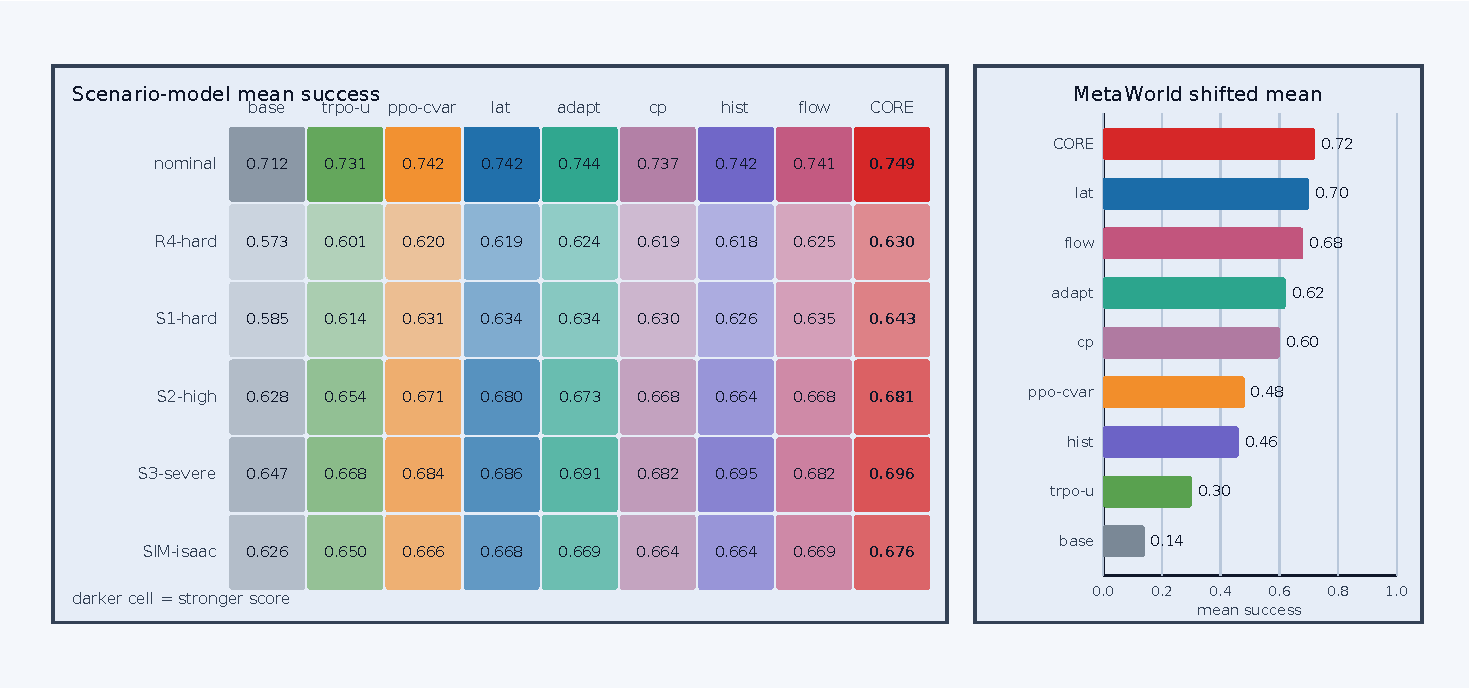
\includegraphics[width=\columnwidth]{figures/recent_baselines_matrix.pdf}
\caption{Coverage view: scenario-model mean-success matrix (left) and shifted MetaWorld mean-success ranking (right) across baseline-family methods and CORE. In the matrix, bold numbers mark the best method per scenario row.}
\label{fig:recent-baselines-matrix}
\end{figure}

This controlled scenario track is for mechanism diagnostics under matched conditions, with floor metrics prioritized in a ceiling regime. Table~\ref{tab:main-results} and Table~\ref{tab:targeted-scenario} show positive deltas for our method versus \CoreProfileExtTwo\ at $N=\CoreCustomSeedN$, targeted $N=\CoreSeedExpN$, and full $N=\CoreExpandedSeedCount$ (\CoreFullNFourteenDeltaExtTwo, CI95 $\pm\CoreFullNFourteenDeltaExtTwoCi$, $p<\CorePermUpperBoundSci$); recent-baseline stress deltas remain Holm-significant.

\begin{table}[t]
\centering
\caption{Controlled scenario-model comparison (\CoreMainSeedCount\ seeds; floor-first).}
\label{tab:main-results}
\begin{tabular}{lcccc}
\toprule
Method & Worst $\uparrow$ & CVaR$_{\CoreCvarPercentLabel}\uparrow$ & Mean $\uparrow$ & CI95 \\
\midrule
Baseline & \CoreCustomBaselineWorst & \CoreCustomBaselineCvar & \CoreCustomBaselineMean & $\pm$\CoreCustomBaselineCi \\
\CoreRefOneLabel & \CoreCustomExtOneWorst & \CoreCustomExtOneCvar & \CoreCustomExtOneMean & $\pm$\CoreCustomExtOneCi \\
\CoreRefTwoLabel & \CoreCustomExtTwoWorst & \CoreCustomExtTwoCvar & \CoreCustomExtTwoMean & $\pm$\CoreCustomExtTwoCi \\
\textbf{CORE} & \textbf{\CoreCustomMethodWorst} & \textbf{\CoreCustomMethodCvar} & \textbf{\CoreCustomMethodMean} & $\pm$\CoreCustomMethodCi \\
\bottomrule
\end{tabular}
\end{table}

Mean gains versus \CoreProfileExtTwo\ are modest, but floor behavior is stronger: worst-seed (\CoreCustomMethodWorst\ vs \CoreCustomExtTwoWorst), CVaR$_{\CoreCvarPercentLabel}$ (\CoreCustomMethodCvar\ vs \CoreCustomExtTwoCvar), and tail-event counts at threshold \CoreTailThreshold\ (\CoreTailNFiveMethod/\CoreTailNFiveDenominator\ vs \CoreTailNFiveExtTwo/\CoreTailNFiveDenominator; at $N=\CoreExpandedSeedCount$: \CoreTailNFourteenMethod/\CoreTailNFourteenDenominator\ vs \CoreTailNFourteenExtTwo/\CoreTailNFourteenDenominator, CVaR delta \CoreTailNFourteenCvarDelta).

\begin{figure}[t]
\centering
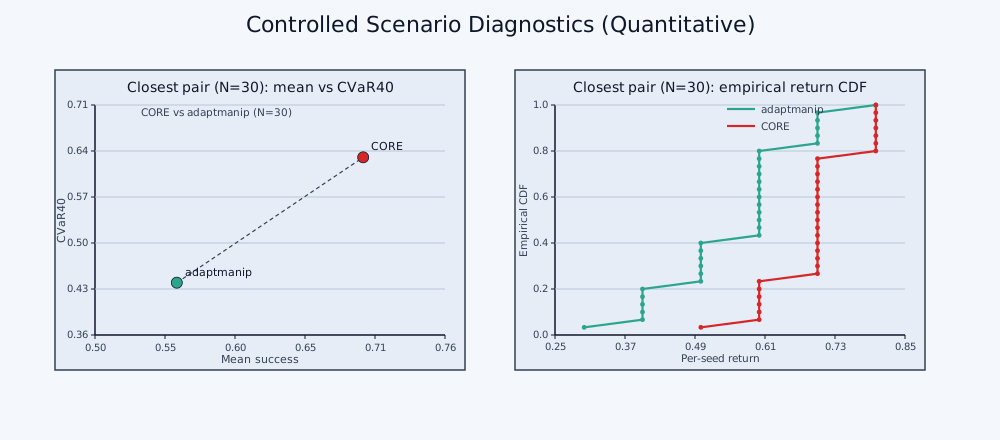
\includegraphics[width=\columnwidth]{../output/corepaper_assets/figures/custom_diagnostics.png}
\caption{Closest-pair diagnostics: mean-vs-CVaR$_{\CoreCvarPercentLabel}$ and deep-$N$ empirical return CDF (\CoreCompAdaptManip\ vs CORE).}
\label{fig:custom-diagnostics}
\end{figure}

Ablations preserve ranking. At \CoreMainSeedCount\ seeds, the full method is \CoreAblationFullMean; no-gate is \CoreAblationNoGateMean\ (\CoreAblationNoGateDelta), no-robust is \CoreAblationNoRobustMean\ (\CoreAblationNoRobustDelta), no-history is \CoreAblationNoHistoryMean\ (\CoreAblationNoHistoryDelta, largest single-factor drop), and no-history+no-gate is \CoreAblationNoHistoryNoGateMean\ (\CoreAblationNoHistoryNoGateDelta). The gate-history interaction residual is \CoreAblationGateHistoryInteractionDelta\ (\CoreAblationGateHistoryInteractionLabel), supporting the gate as a complementary tail-risk filter. Independent rerun streams yield a small full-method mean gap (\CoreAblationVsMainMethodMeanGap).

Our method meets stress criteria and remains ahead in sim-to-sim transfer (\CoreEnvMujoco$\rightarrow$\CoreEnvIsaac, \CoreSimSeedCount\ seeds/variant), with target retention \CoreSimIsaacMethodRetentionPct\% (average per-seed transfer ratio; not exact ratio-of-means; Table~\ref{tab:sim2sim}). Evidence is software-only (no hardware runs).

\begin{table}[t]
\centering
\caption{Sim-to-sim transfer summary (\CoreSimSeedCount\ seeds per engine and variant; primary lanes only).}
\label{tab:sim2sim}
\resizebox{\columnwidth}{!}{%
\begin{tabular}{lcccc}
\toprule
Engine & Baseline & \CoreRefTwoLabel & CORE & CORE retention (\%) \\
\midrule
Mujoco (source) & \CoreSimMujocoBaselineMean & \CoreSimMujocoExtTwoMean & \CoreSimMujocoMethodMean & \CoreSimMujocoMethodRetentionPct \\
Isaac (target) & \CoreSimIsaacBaselineMean & \CoreSimIsaacExtTwoMean & \CoreSimIsaacMethodMean & \CoreSimIsaacMethodRetentionPct \\
\bottomrule
\end{tabular}
}
\end{table}

Uncertainty diagnostics are stable (cu=\CoreUncertaintyCu, c0=\CoreUncertaintyCzero, MAE=\CoreUncertaintyHoldoutMae, max Assump.-2 violation=\CoreUncertaintyMaxViolation\ on [0,1]). Calibration uses a disjoint split (\CoreUncertaintyTrainRows\ fit, \CoreUncertaintyHoldoutRows\ holdout) with holdout Assump.-2 coverage \CoreUncertaintyCoveragePct\%. \CoreCompAdaptManip\ one-sided condition violation is \CoreUncertaintyViolationRate\ (\CoreUncertaintyViolationRatePct\%); deployment uses only the two-sided gate.

\section{Discussion and Limitations}

Limitations: evidence is simulation-only, failures cluster under severe co-shift, and sim-to-real drift remains untested. Closest-comparator fairness also has a scope caveat: \CoreCompAdaptManip\ uses a pinned in-repo profile, not an official-library parity audit. Adaptive threshold tuning remains an operational burden across regimes; we mitigate this with fixed quantile defaults and report misspecification sensitivity diagnostics. Sim-to-sim transfer retains \CoreSimIsaacMethodRetentionPct\% on Isaac, but hardware robustness remains future work.

\section{Conclusion}
Our approach frames robust policy updating as an online control problem: optimize a risk-aware objective, then commit candidate updates only when uncertainty-gated checks support deployment. Across matched-seed shift evaluations, this promote/monitor/rollback design improves reliability-floor behavior while preserving fixed-budget update control, with the clearest benefit in adverse-tail regimes where unstable updates are most costly.

The evidence also clarifies scope boundaries. Primary confirmatory claims are anchored to \CoreRefTwoLabel, while \CoreCompAdaptManip\ remains a paper-profile exploratory lane rather than official-library parity evidence. Results are simulation-only, and severe co-shift settings remain the dominant failure mode.

Taken together, the study supports uncertainty-gated update control as a practical reliability mechanism for shift-aware policy optimization, and it motivates three immediate next steps: official-code comparator parity for closest baselines, hardware validation under real-world drift, and more adaptive-yet-auditable threshold selection policies.

\bibliographystyle{IEEEtran}
\bibliography{references}

\end{document}
